%************************************************
\chapter{ControlBO: Bayesian Optimization for Controller Tuning}\label{ch:mfbo} 
%************************************************

\section{Introduction}
\label{sec:intro}
Laboratory unit operations such as reactors and distillation columns  are often subjected to many processes in a short window of time. For each new process, the control systems of these unit operations need to be re-tuned, which can be a time and labor intensive endeavor. As an example, in the distillation laboratories at BASF, operators often spend days attempting to find the best tuning parameters for a new distillation column setup, which is unacceptable given the short timelines of operating a testing laboratory. While it is possible to use model predictive control, decentralized PID controllers are often used due to their robustness and simplicity. In this chapter, I aim to develop a fast method for tuning controllers and apply this method laboratory distillation columns.

As noted in Chapter \ref{ch:rl_tuning}, there are a wide variety of existing tuning protocols ranging from heuristics such as Ziegler Nichols \cite{Ziegler1942} and its refinements \cite{Hang1991} to tuning using analytical equations from models via methods such as  Internal Model Control \cite{Copeland2010}. However, extending these to multi-input multi-output systems has been challenging, often requiring additional optimizations \cite{Nandong2013, Nandong2015}. Optimization-based methods have shown promise \cite{Pajares2019, Sumana2010, Rajapandiyan2012, Behroozsarand2012}, but these methods have been difficult to apply in practice due to the large number of iterations they require. Recently, Bayesian optimization (BO) has shown promise for tuning controllers \cite{NeumannBrosig2020, Fiducioso2019, Khosravi2020, Konig2020, Fujimoto2022, Brunzema2022, Khosravi2022}, but this method still often requires tens to hundreds of iterations, making it too materially expensive for laboratory chemical processes.

One approach to reduce the number of iterations required for BO is multifidelity Bayesian optimization (MFBO). MFBO leverages data from an auxiliary simulation or data source that is faster or cheaper to evaluate. Early examples of this approach include Kennedy et al. who used low fidelity approximations of an oil rig simulation to reduce the number of calls to a slower simulator \cite{Kennedy2000}. More recently , multifidelity Bayesian optimization approaches have developed to accelerate the tuning of hyperparameters for machine learning models \cite{pmlr-v70-kandasamy17a}, design of batteries \cite{Folch2023} and optimization of airplane rotors \cite{Pan2017}. Readers should refer to Chapter \ref{ch:background} for review of multifidelity and transfer learning in Bayesian optimization.

In this chapter, I use Bayesian optimization to accelerate controller tuning. Specifically, I develop a dynamic simulation of a distillation column that is low fidelity approximation of the original distillation experiment. I then introduce a novel BO strategy called ControlBO designed specifically for tuning control systems and explore whether multifidelity BO can accelerate controller tuning.

\begin{figure}
    \centering
    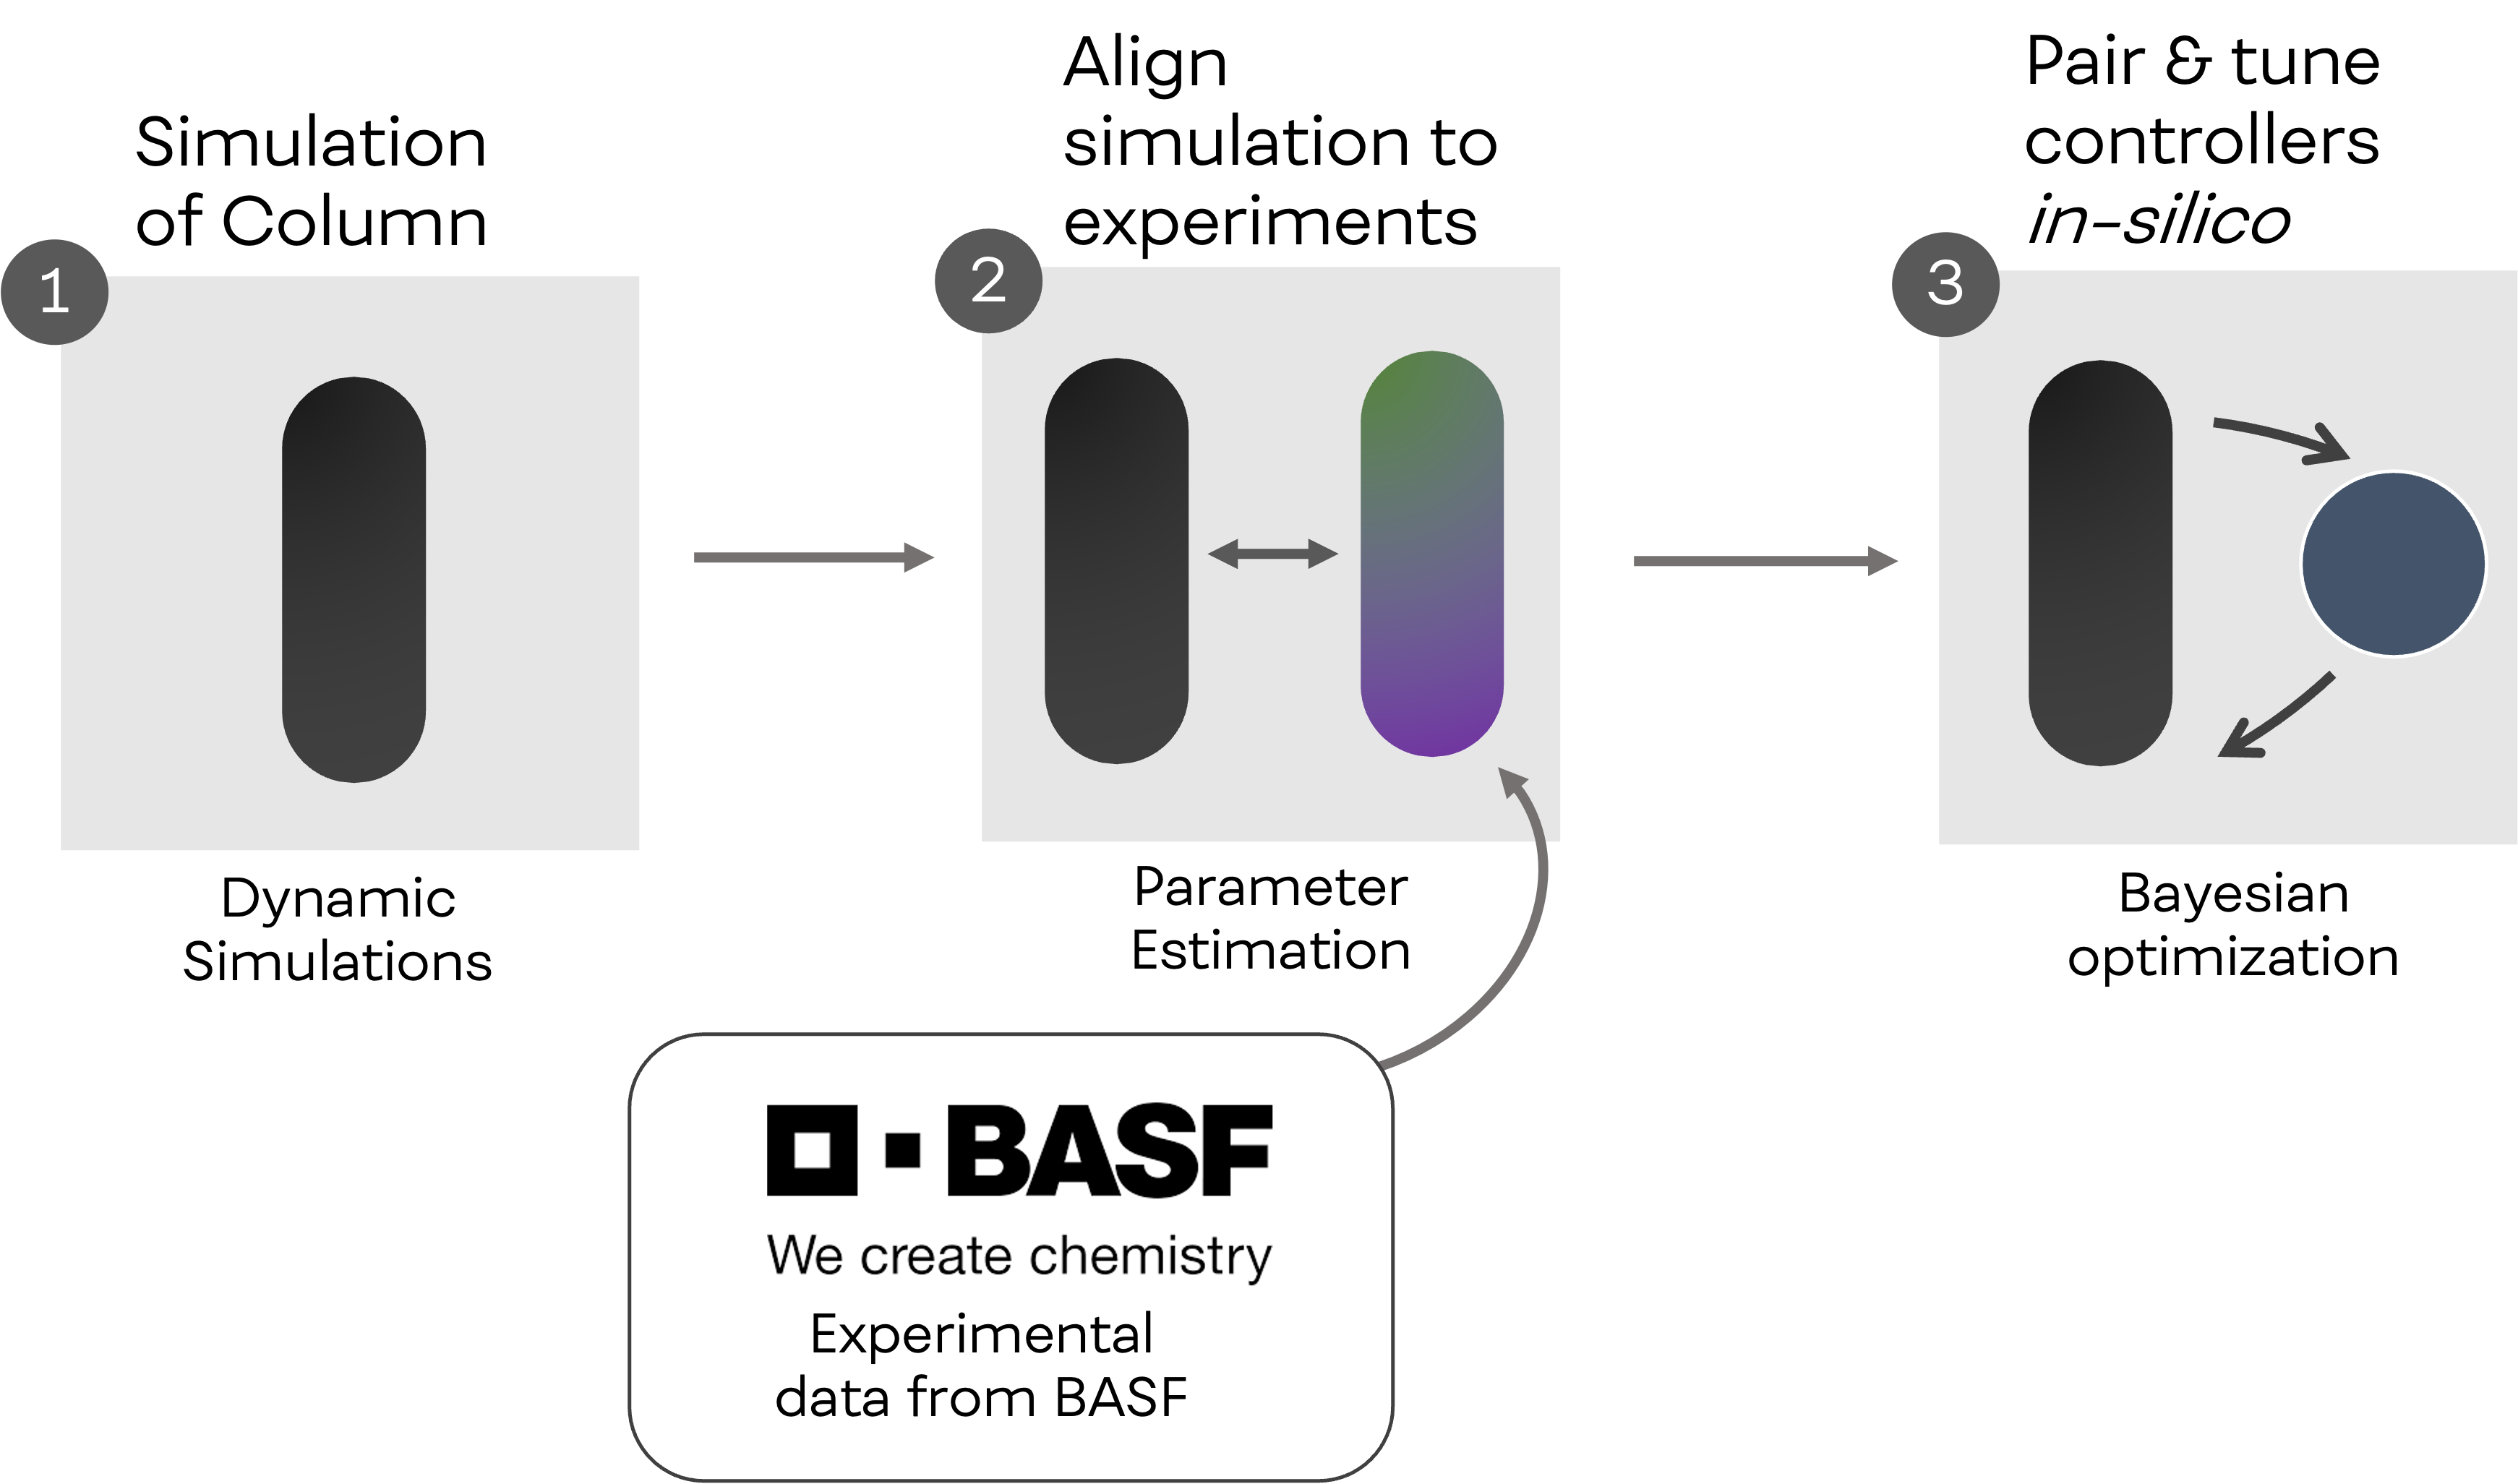
\includegraphics[width=0.8\textwidth]{gfx/Chapter06/tuning_workflow.png}
    \caption{Three step workflow for distillation controller design and tuning.}
    \label{fig:tuning_workflow}
\end{figure}

\section{Methods}

\subsection{Controller tuning as an optimization problem}

As noted in Chapter \ref{ch:rl_tuning}, controller tuning involves identifying the three parameters of the PID equation, $K^P$, $\tau_I$ and $\tau_D$:

\begin{equation}
    u(t) = PI(Y, Y^{sp}, \Omega) =  K^P e(t) + \frac{1}{\tau_I}\int_0^t e(t')dt' + \tau_D \frac{de(t)}{dt}
\end{equation}
\begin{equation}
    e(t) = (Y^{sp} - Y)
\end{equation}
where $u(t)$ is the controller output that is feed into the actuator (e.g., a valve) and $e(t)$ is the error at time $t$. $Y$ is the controlled variable, and $Y^{sp}$ is the setpoint, and $\Omega=\{K^p, \tau_I, \tau_D \}$ are the controller parameters. In this work, I only use PI controllers, so $\tau_D=0$.

I formulate the problem of controller design and tuning as an optimization problem. The aim is to find a set of controller parameters that will achieve desired behavior. I define good controller behavior as minimizing the integral absolute error (IAE) for each controlled variable and minimizing total controller movement (CM):
\begin{equation}
    \min_{\Omega}(IAE_1, IAE_2, IAE_3, CM_1, CM_2, CM_3)
\end{equation}


\begin{equation}
    IAE = \int_0^T \vert y_{sp}(t) - \hat y(t) \vert dt
\end{equation}

\begin{equation}
    CM = \sum_{t=1}^{T}( \vert x_t - x_{t-1} \vert)
\end{equation}
where $y_{sp}$ is the setpoint,  $\hat y$  is the value of  the variable, T is the time horizon. 

\subsection{ControlBO: Bayesian optimization for controller tuning}

ControlBO is a Bayesian optimization algorithm that aims to identify robust controller parameters for MIMO systems in as few experiments as possible. I was inspired by a recent paper by Paulson et al. that uses a Gaussian Process to model both the uncertain variables as well as the controller parameters \cite{Paulson2022}. They then use min-max formulation where the integral absolute error is minimized, while the uncertain variables are held at their maximum value. However, they sample from a high fidelity simulation and then assume that this simulation will always transfer to laboratory experiments.

ControlBO is a multifidelity and multi-objective Bayesian optimization algorithm that aims to solve the following problem:

\begin{equation}
    \Omega^* = \min_{\Omega} \mathbf f(\Omega, x, \delta)
\end{equation}
where $\Omega$ are the controller parameters and $\mathbf f$ is the laboratory controller tuning problem. $\delta$ are disturbance variables that might be stepped by operators or changed by other external factors. Similar to Paulson et al. \cite{Paulson2022}, I use a min max formulation where a GP is trained on both controller parameters $\Omega$ and values of disturbance variables from past tuning experiments. During acquisition function optimization, the disturbance variables are fixed at their maximum value, while the controllers parameters are varied to maximize the acquisition function. Fixing the disturbance variables ensures that robust controller parameters are chosen.

ControlBO trains an independent multitask GP to predict each controller objective (IAE) and controller movement (CM) given the relevant controller parameters. The multitask GP is trained on both auxiliary simulation data and tuning experiments. This is what makes ControlBO multifidelity.

Since our problem is multi-objective, I used a multi-objective acquisition function, namely the q Expected Hypervolume Improvement (qEHVI) \cite{Balandat2020}. This acquisition function has a balance of computational efficiency and fidelity resulting in an ability to find the Pareto front of trade-offs between objectives quickly. 

I developed a differential equation simulation of a distillation column that was aligned to experimental data using both steady state and dynamic parameter estimation. To leverage the simulation, I used a multi-task GP that could be trained on both the less abundant high fidelity experimental data and the more abundant low fidelity simulation data. I hoped that the multi-task GP could learn the correlation between the simulation and the experimental data and thus make better predictions on the experiments with less data.

% Additionally, I found that the simulations often failed with certain controller parameters. Therefore, I trained a classifier to predict the likelihood of a successful simulation, which I expect to also correlate with reasonable experimental parameters. The probability of success predicted by the classifier was multiplied by the qNEHVI acquisition function value to form a chance constrained acquisition function:

% \begin{equation}
%     \alpha_{cc} = p(h \vert \mathcal D) \alpha_{qNEHVI}
% \end{equation} 

In practice, I optimized the high fidelity task when selecting  a new set of controller parameters ton run an experiment in the laboratory. Then, while waiting for the laboratory results, I optimized the lower fidelity task using the differential equation simulation with the most recently estimated parameters. 

\subsection{Distillation Simulation}\label{sec:distillation_model}

In order to base our simulations in reality, my collaborators at BASF collected experimental data for separation of a 50/50 methanol-water mixture at the laboratories of BASF SE in a 80 tray column with one bubble cap on each stage. The column was kept at approximately 800 mbar vacuum, and a Julabo evaporator was used as the reobiler. The column occupies approximately three stories in the BASF lab.  

% Three days of data were collected, one of which is used for parameter estimation and the rest for validation. 

My goal in simulating a distillation columns was to find a balance between model complexity and accuracy. I opted for a formulation similar to \citet{Diehl2001}, which assumes constant pressure drop over time but includes the MESH equations and hydrodynamics. As shown in Figure \ref{fig:column}, $N$ is the number of trays in the distillation column. The distillation column is numbered from the bottom, starting with the reboiler as $i=0$ and condenser as $i=N+1$.  

\begin{figure}
    \centering
    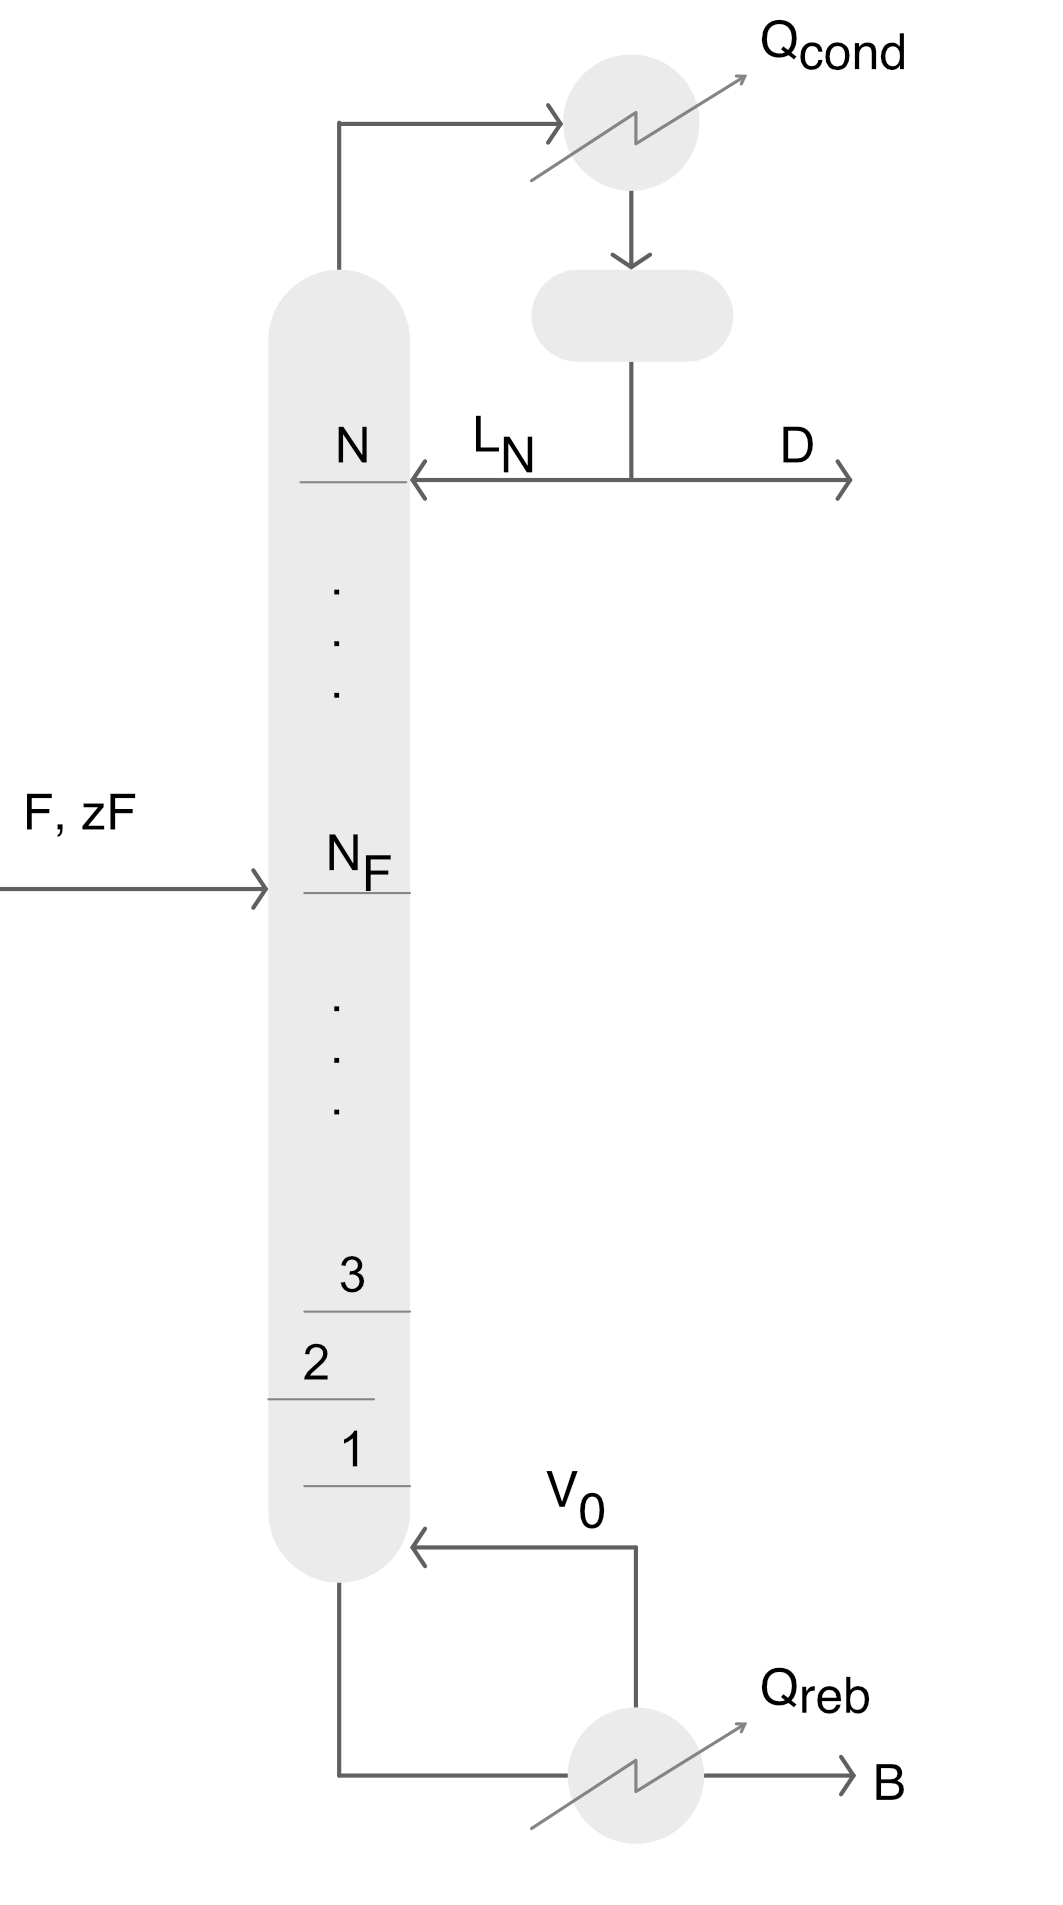
\includegraphics{gfx/Chapter06/basic_column.png}
    \caption{Depiction of a distillation column with $N$ trays, feed at stage $N_F$, and reboiler and condenser as stage 0 and $N+1$ respectively.}
    \label{fig:column}
\end{figure}


% The following are parameters of the model, determined by the experimental scenario or estimated via parameter estimation (see the next section).

% \begin{itemize}
%     \item$P_{top}$ is the pressure above stage $N$ in the column
%     \item$\Delta P_{strip}$ is the pressure drop in the stripping section (below feed stage)
%     \item$\Delta P_{rect}$ is the pressure drop in the rectifying section (feed stage and above)
%     \item$q_{N_F}$ is the vapor fraction in the feed
%     \item$z_{N_F}$ is the mol fraction in the feed
%     \item$F$ is the feed flowrate (kmol/hr)
%     \item$Q_{reb}$ is reboiler duty
%     \item$Q_{cond}$ is the condenser duty
%     \item$\alpha_{strip}$ is the Murphree efficiency in the stripping section (below feed stage)
%     \item$\alpha_{rect}$ is the Murphree efficiency in the rectifying section (feed stage and above)
% \end{itemize}

assumed the pressure drop was constant throughout the simulation, which is reasonable given the experimental observations (a vacuum was used to keep pressure drop constant). Therefore the pressure on each stage is calculated using:

% \begin{table}
%     \centering
%     \caption{Parameters of the distillation column model determined by experiments.}
%     \begin{tabular}{cccc}
%         \textbf{Parameter} & \textbf{Description} & \textbf{Scenario 1} & \textbf{Scenario 2}  \\
%         \hline
%          $P_{top}$ &  Pressure on stage N of the column &  0.5 & 0.22 \\ 
%          $q_{N_F}$ & vapor fraction  in the feed & 1.0 & 1.0 \\
%          $z_{N_F}$  & mole fraction of methanol in the feed &  0.5  & 0.5 \\
%          $F$ & Feed flow rate &  333 mol/min  & 332 mol/min \\
%          \hline
%     \end{tabular}
%     \label{tab:parameters}
% \end{table}

\begin{equation}
    P_i = P_{i+1} + \Delta P_i \;\; i=0\dots N
\end{equation}

where $\Delta P_i =\Delta P_{strip}$ for stages below feed stage and $\Delta P_i =\Delta P_{rect}$ for feed stage and above. The condenser pressure is calculated using $P_{cond}=P_{N} - \Delta P_{rect}$.

Constant parameters are shown in Table \ref{tab:parameters} and state variables in Table \ref{tab:state_variables}.
\begin{table}
    \centering
    \caption{State variables of the distillation column model.}
    \begin{tabular}{cc}
        \textbf{Variabe} & \textbf{Description}  \\
        \hline
         $x_i$ &  Liquid composition of methanol on stage $i$ \\
         $y_i$ & Vapor composition of water on stage $i$\\
         $L_i$ & Liquid flow on stage $i$  \\
         $V_i$  & Vapor flow on stage $i$ \\
         $T_i$  & Temperature on stage $i$ \\
         $T_i$  & Holdup on stage $i$ \\
         \hline
    \end{tabular}
    \label{tab:state_variables}
\end{table}

\subsubsection{Material balances}
Material balances are calculated for all stages as follows:

\begin{equation}
\frac{dn_i}{dt} = L_{i+1}-L_i + V_{i-1}-V_i \;\; \forall i=1 \dots N_F-1, N_F+2 \dots N+1
\end{equation}

Note that the feed stage and the stage above the feed stage are treated separately:

\begin{equation}
    \frac{dn_{N_F}}{dt} = L_{N_F+1}-L_{N_F} + V_{N_F-1}-V_{N_F} + q_{N_F}F   
\end{equation}

\begin{equation}
   \frac{dn_{N_F+1}}{dt} = L_{N_F+2}-L_{N_F+1} + V_{N_F}-V_{N_F+1} + (1-q_{N_F})F 
\end{equation}

where $q_i$ is the liquid fraction of the feed stream.

The material balance for the sump:

\begin{equation}
    \frac{dn_1}{dt} = L_2 - L_1 + V_0 - V_1
\end{equation}

I assume that the holdup in the thermosyphon reboiler is constant over time, and that all liquid flowing into the reboiler is vaporized. Therefore, the liquid flow into the reboiler is equal to the vapor flow out of the reboiler $V_0$, resulting in the following balance at the bottom of the sump:
\begin{equation}
    L_0 = V_0 + B
\end{equation}

The condenser and reflux drum are lumped and consider as one unit.

\begin{equation}
    \frac{dn_{N+2}}{dt} = V_{N+1}-(L_{N+2} + D)    
\end{equation}


\subsubsection{Component balances}

Component balances are calculated for all trays:
\begin{equation}
   \frac{d(x_{i} n_{i})}{dt}= L_{i+1} x_{i+1} - L_i x_{i} + V_{i-1} y_{i-1} -V_i y_i  \;\; \forall i=1 \dots N_F-1, N_F+2 \dots N+1
\end{equation}

The  feed stage and the stage above the feed stage are treated separately:

\begin{equation}
\begin{split}
 \frac{d(x_{N_F} n_{N_F})}{dt} =  &  x_{N_F+1}L_{N_F+1}  - x_{N_F}L_{N_F} +  y_{N_F-1}V_{N_F-1} \\ & -y_{N_F}V_{N_F} + q_{N_F}z_FF   
\end{split}
\end{equation}

\begin{equation}
\begin{split}
    \frac{d(x_{N_F+1} n_{N_F+1})}{dt} =  & x_{N_F}L_{N_F} - x_{N_F+1}L_{N_F+1} +  y_{N_F+2}V_{N_F+2}   \\ & -y_{N_F+1}V_{N_F+1}  + (1-q_{N_F})z_FF 
\end{split}
\end{equation}

Given the previously stated assumption of a total reboiler, the composition of the liquid and vapor in the reboiler are the same:

\begin{equation}
    x_0 = y_0
\end{equation}

The component balance around the sump is as follows:

\begin{equation}
    \frac{d(x_{0} n_{0})}{dt} = L_2 x_2 - L_1 x_1 + V_0 y_0 - V_1 y_1
\end{equation}

The component balance around the condenser is as follows:
\begin{equation}
    \frac{d(x_{N+2} n_{N+2})}{dt}  = V_{N+1} y_{N+1} - x_{N+2} (L_{N+2} + D)
\end{equation}

\subsubsection{Energy balances}\label{sec:energy_balances}

In calculating energy balances, I assume that vapor holdup is negligible and therefore only consider the liquid holdup. Energy balances are calculated using the liquid and vapor enthalpy, as detailed subsequently. For the trays:

\begin{equation}
\begin{split}
    \frac{d(n_ih^L_i)}{dt} = h^L_{i+1}L_{i+1}-h^L_iL_i+h^V_{i-1}V_{i-1}-h^V_iV_i + Q_i  \\ \forall i=1 \dots N_F-1, N_F+2 \dots N+1
\end{split}
\end{equation}

For the feed stage and the stage above the feed stage:

\begin{equation}
\begin{split}
    \frac{d(n_{N_F}h^L_{N_F})}{dt} = & h^L_{N_F+1}L_{N_F+1}-h^L_{N_F}L_{N_F} + h^V_{N_F-1}V_{N_F-1}-h^V_{N_F}V_{N_F} \\ &  + q_{N_F}F h^L_{N_F}
\end{split}
\end{equation}


\begin{equation}
\begin{split}
    \frac{d(n_{N_F+1}h^L_{N_F+1})}{dt} = & h^L_{N_F+2}L_{N_F+2}-h^L_{N_F+1}L_{N_F+1} +h^V_{N_F} V_{N_F}-\\ &h^V_{N_F+1} V_{N_F+1} + (1-q_{N_F})Fh^V_{N_F}
\end{split}
\end{equation}

 The energy balances for the reboiler and sump respectively are:

\begin{equation}
    \frac{d(n_0h^L_0)}{dt} = V_0(h^L_{1} - h^V_0) + Q_0
\end{equation}

\begin{equation}
    \frac{d(n_1h^L_1)}{dt} = L_2 h^L_2 - L_1 h^L_1 + V_0 h^V_0 - L_1 h^L_1 + Q_1  
\end{equation}

The energy balance for the condenser is as follows:

\begin{equation}
    \frac{d(n_{N+2}h^L_{N+2})}{dt} = h^V_{N+1} V_{N+1}-h^L_{N+2}(L_{N+2} + D) + Q_{N+2}
\end{equation}

Additionally, a heat exchanger subcools the liquid from the condenser:

\begin{equation}
    n_{subcool}\frac{d h^L_{reflux}}{dt} = L_{N+2}(h^L_{N+2} - h^L_{reflux}) + Q_{subcool}
\end{equation}

For liquid enthalpy $h^{L,c}$ of each component, take a mole fraction weighted average of the specific enthalpies calculated by integrating a constant heat capacity from a reference temperature $T_{ref}$ of normal boiling point of each component $c$. Data is taken from Table 2-72 of Perry’s Chemical Engineering Handbook \cite{Perrys2018}.

\begin{equation}
    h^L(T_i, P_i, x_i) = x_ih^{L,0}(T_i,P_i) + (1-x_i)h^{L,1}(T_i,P_i)
\end{equation}

\begin{equation}
    h^{L,c}(T,P) = \int_{T_{ref}}^T C_p^c(\tau)d\tau 
\end{equation}

\begin{equation}
    C_p^c(T) = \sum_{k=0}^5 c^kT^k 
\end{equation}

The enthalpy of the liquid on stage $i$ is then:
\begin{equation}
    h^L_i := h^L(T_i, P_i,x_i)
\end{equation}

\begin{equation}
    h^L_{N_F} := h^L(T_{N_F}, P_{N_F},x_{N_F})
\end{equation}

For vapor enthalpy,  a similar approach is taken. Data for heat of vaporization and vapor enthalpy is taken from Table 2-169 and Table 2-102 respectively in Perry’s Chemical Engineering Handbook \cite{Perrys2018}.

\begin{equation}
    h^V(T_i, P_i, x_i) = x_i h^{V,0}(T_i,P_i) + (1-x_i) h^{V,1}(T_i,P_i)
\end{equation}


\begin{equation}
    h^{V,c}(T,P) = H^{vap, c}(T_{ref}) + 4R(T-T_{ref})
\end{equation}

\begin{equation}
    h^V_i := h^V(T_i, P_i,x_i)
\end{equation}

\begin{equation}
    h^V_{N_F} := h^V(T_{N_F}, P_{N_F},x_{N_F})
\end{equation}


\subsubsection{Activity coefficient model}

I use the NRTL model for calculating the activity coefficients, though a variety of models could be used. The NRTL parameters for methanol-water are shown in Table \ref{tab:nrtl_parameters}.

\begin{table}[]
    \centering
    \caption{Methanol-water NRTL parameters. Taken from Beneke et al.\cite{Beneke2012}}
    % https://onlinelibrary.wiley.com/doi/pdf/10.1002/9781118477304.app2
    \begin{tabular}{cc}
        Parameter & Value \\
        \hline
         $\tau_{12}$ & -0.693  \\
         $\tau_{21}$ & 2.732   \\
         $\alpha_{12}$ & 0.3 \\
    \end{tabular}
    \label{tab:nrtl_parameters}
\end{table}

\begin{equation}
    \ln \gamma_{i,0} = x_2^2\biggl [\tau_{21} \biggl (\frac{G_{21}}{x_1+x_2G_{21}}\biggr)^2 + \frac{\tau_{12}G_{12}}{(x_2 + x_1 G_{12})^2} \biggr ]
\end{equation}

\begin{equation}
     \ln \gamma_{i,1} = x_1^2\biggl [\tau_{12} \biggl (\frac{G_{12}}{x_2+x_1G_{12}}\biggr)^2 + \frac{\tau_{21}G_{21}}{(x_1 + x_2 G_{21})^2} \biggr ]   
\end{equation}

\subsubsection{Pressure balance}

Vapor pressure is calculated using Antoine’s equation with coefficients taken from NIST. 

\begin{equation}
    \log P_{i,k}^{sat}(T_i) = A_k + \frac{B_k}{T_i + C_k}
\end{equation}

For trays ($i=1\dots N$), modified Raoult’s Law is used with Murphree efficiencies to account for deviations from equilibrium.

\begin{equation}
    y_i = \alpha_i\frac{x_i\gamma_i(T_i, P_i, x_i)P_0^{sat}(T_i)}{P} + (1-\alpha_i)y_{i-1}
\end{equation}

This leads to the bubble pressure balance:

\begin{equation}
    P = x_i\gamma_{i,0}(T_i, P_i, x_i)P^{sat}_{i,0} + (1-x_i)\gamma_{i,1}(T_i, P_i, (1-x_i))P^{sat}_{i,1}
\end{equation}

\subsubsection{Francis weir formula}

The Francis weir formula is used for dynamic simulations to calculate liquid flow over the weir given a certain holdup. As shown in Figure \ref{fig:weir}, $h_i^{ow}$ from the the clear liquid to the weir. can calculate this by taking the difference between the actual volume in the weir and a reference volume $n^v_{ref}$ (i.e., the volume if there was no crest) given the cross sectional area.

\begin{figure}
    \centering
    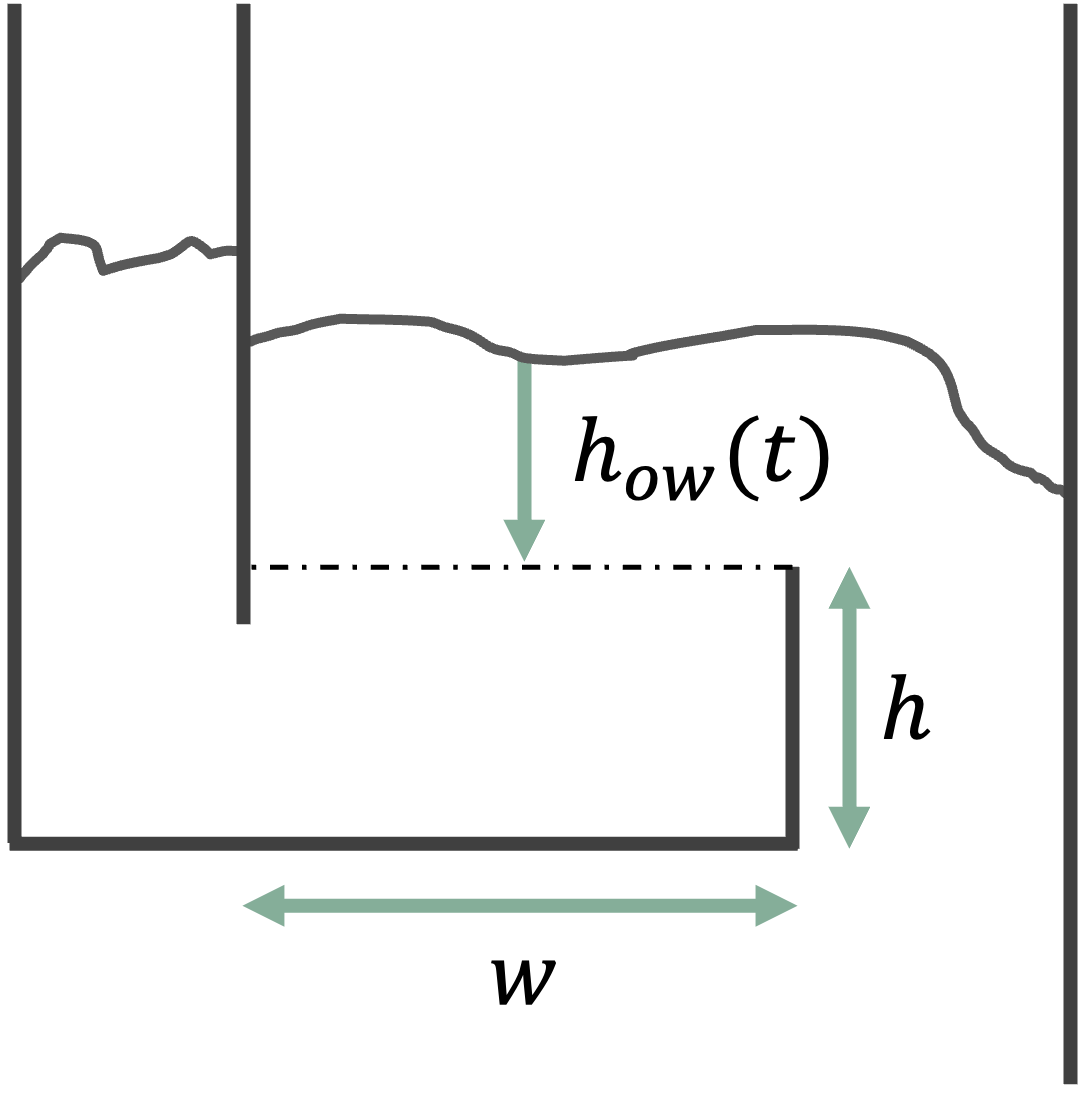
\includegraphics[width=0.4\textwidth]{gfx/Chapter06/weir.png}
    \caption{Diagram of weir showing $h_{ow}$ measured from the top of the clear liquid on a tray.}
    \label{fig:weir}
\end{figure}


\begin{equation}
    h^{ow}_i = \frac{n^v_i-n^v_{ref}}{A}
\end{equation}

The francis Weir formula for calculating flow over the Weir comes from the Bernoulli equation for the horizontal velocity $v$. The equation is integrated from the top of the liquid (y=0) to the weir ($y=h_i^{ow}$)

\begin{equation}
    \frac{1}{2} \rho v^2 = \rho g y \ \Longrightarrow v(y) = \sqrt{2gy}
\end{equation}

\begin{equation}
    L_i^{vol} = \int_0^{h_i^{ow}} v(y)wdy = w\sqrt{2g}\int_0^{h_i^{ow}} y^{1/2}dy = \frac{2}{3}w\sqrt{2g}(h_i^{ow})^{3/2} 
\end{equation}


Substituting for $h_i^{ow}$:

\begin{equation}
   L_i^{vol} = \frac{2}{3} w\sqrt{2g}\biggl(\frac{n^v_i-n^v_{ref}}{A}\biggr)^{3/2}  
\end{equation}

All constants are then lumped into a a single parameter $W_{tray}$:

\begin{equation}
    L_i^{vol} = W_{tray}(n_i^v-n^v_{ref})^{3/2}
\end{equation}

\begin{equation}
    W_{tray} = \frac{2}{3}w\sqrt{2g}A^{-3/2}
\end{equation}

Based on measurements from BASF, assume the diameter of the weir $w$ is 8 mm and the height of the weir $h$ is 10 mm. take $h = 1\cdot10^{-2} m$ and $A=\pi w^2/4 = \pi(8 \cdot 10^{-3})^2/4 = 5.024 \cdot 10^{-5} m^2$, and g is the gravity of Earth. Therefore $W_{tray}^{init}=120149 \; m^{-3/2}s^{-1}$. $n^v_{ref}=Ah=5.024 \cdot 10^{-7} m^3$. 

Since the simulation is in molar flowrates, volumetric flowrates should be converted to molar flowrates:

\begin{equation}
    L_i = \rho(T_i, x_i)L^{vol}_i  
\end{equation}


where $\rho(T_i,x_i)$ is the volumetric density, calculated by a weighted average of the volumetric density of both components. Volumetric density come from Perry’s Chemical Engineering Handbook \cite{Perrys2018}.

\begin{equation}
    \rho(T_i, x_i) = x_i\rho^0(T_i, x_i) + (1-x_i)\rho^1(T_i, x_i)
\end{equation}

\subsubsection{Feedback control}

Three PI controllers are used to control the distillation column. The first two controllers are  level controllers:

\begin{equation}
    D := PI(l_{condenser}, \Omega_{cond})
\end{equation}

\begin{equation}
    B := PI(l_{sump}, \Omega_{sump})
\end{equation}

where $l$ is the level in the respective vessel. The level (\%) is calculated using the following linear equation which is based on data from BASF:

\begin{equation}
    l = c^1 n + c^2
\end{equation}

where $c^1=143.94 m^{-1}$ and $c^2=0.21$.

A composition controller uses the temperature on stage 17 as the controlled variable and the reboiler heat as the manipulated variable.

\begin{equation}
    Q_0 := PI(T_{17}, \Omega_{composition})
\end{equation}

\subsection{Solving and aligning model using GEKKO}

I implemented the equations from the previous section in a simulation of a distillation column that can be aligned to experiments using a small amount of steady state data. The distillation simulation was built in Python using GEKKO \cite{Beal2018}, and the differential algebraic equation model used for the simulations is fully detailed in Section \ref{sec:distillation_model}. To align the simulation to experiments, a three step procedure, illustrated in Figure \ref{fig:simulation_workflow}, was followed: initialization, steady state solution with parameter estimation and dynamic simulation. All simulations were solved with the APOPT nonlinear programming solver to a tolerance $10^{-9}$ and relative tolerance $10^{-9}$.

\begin{figure}
    \centering
    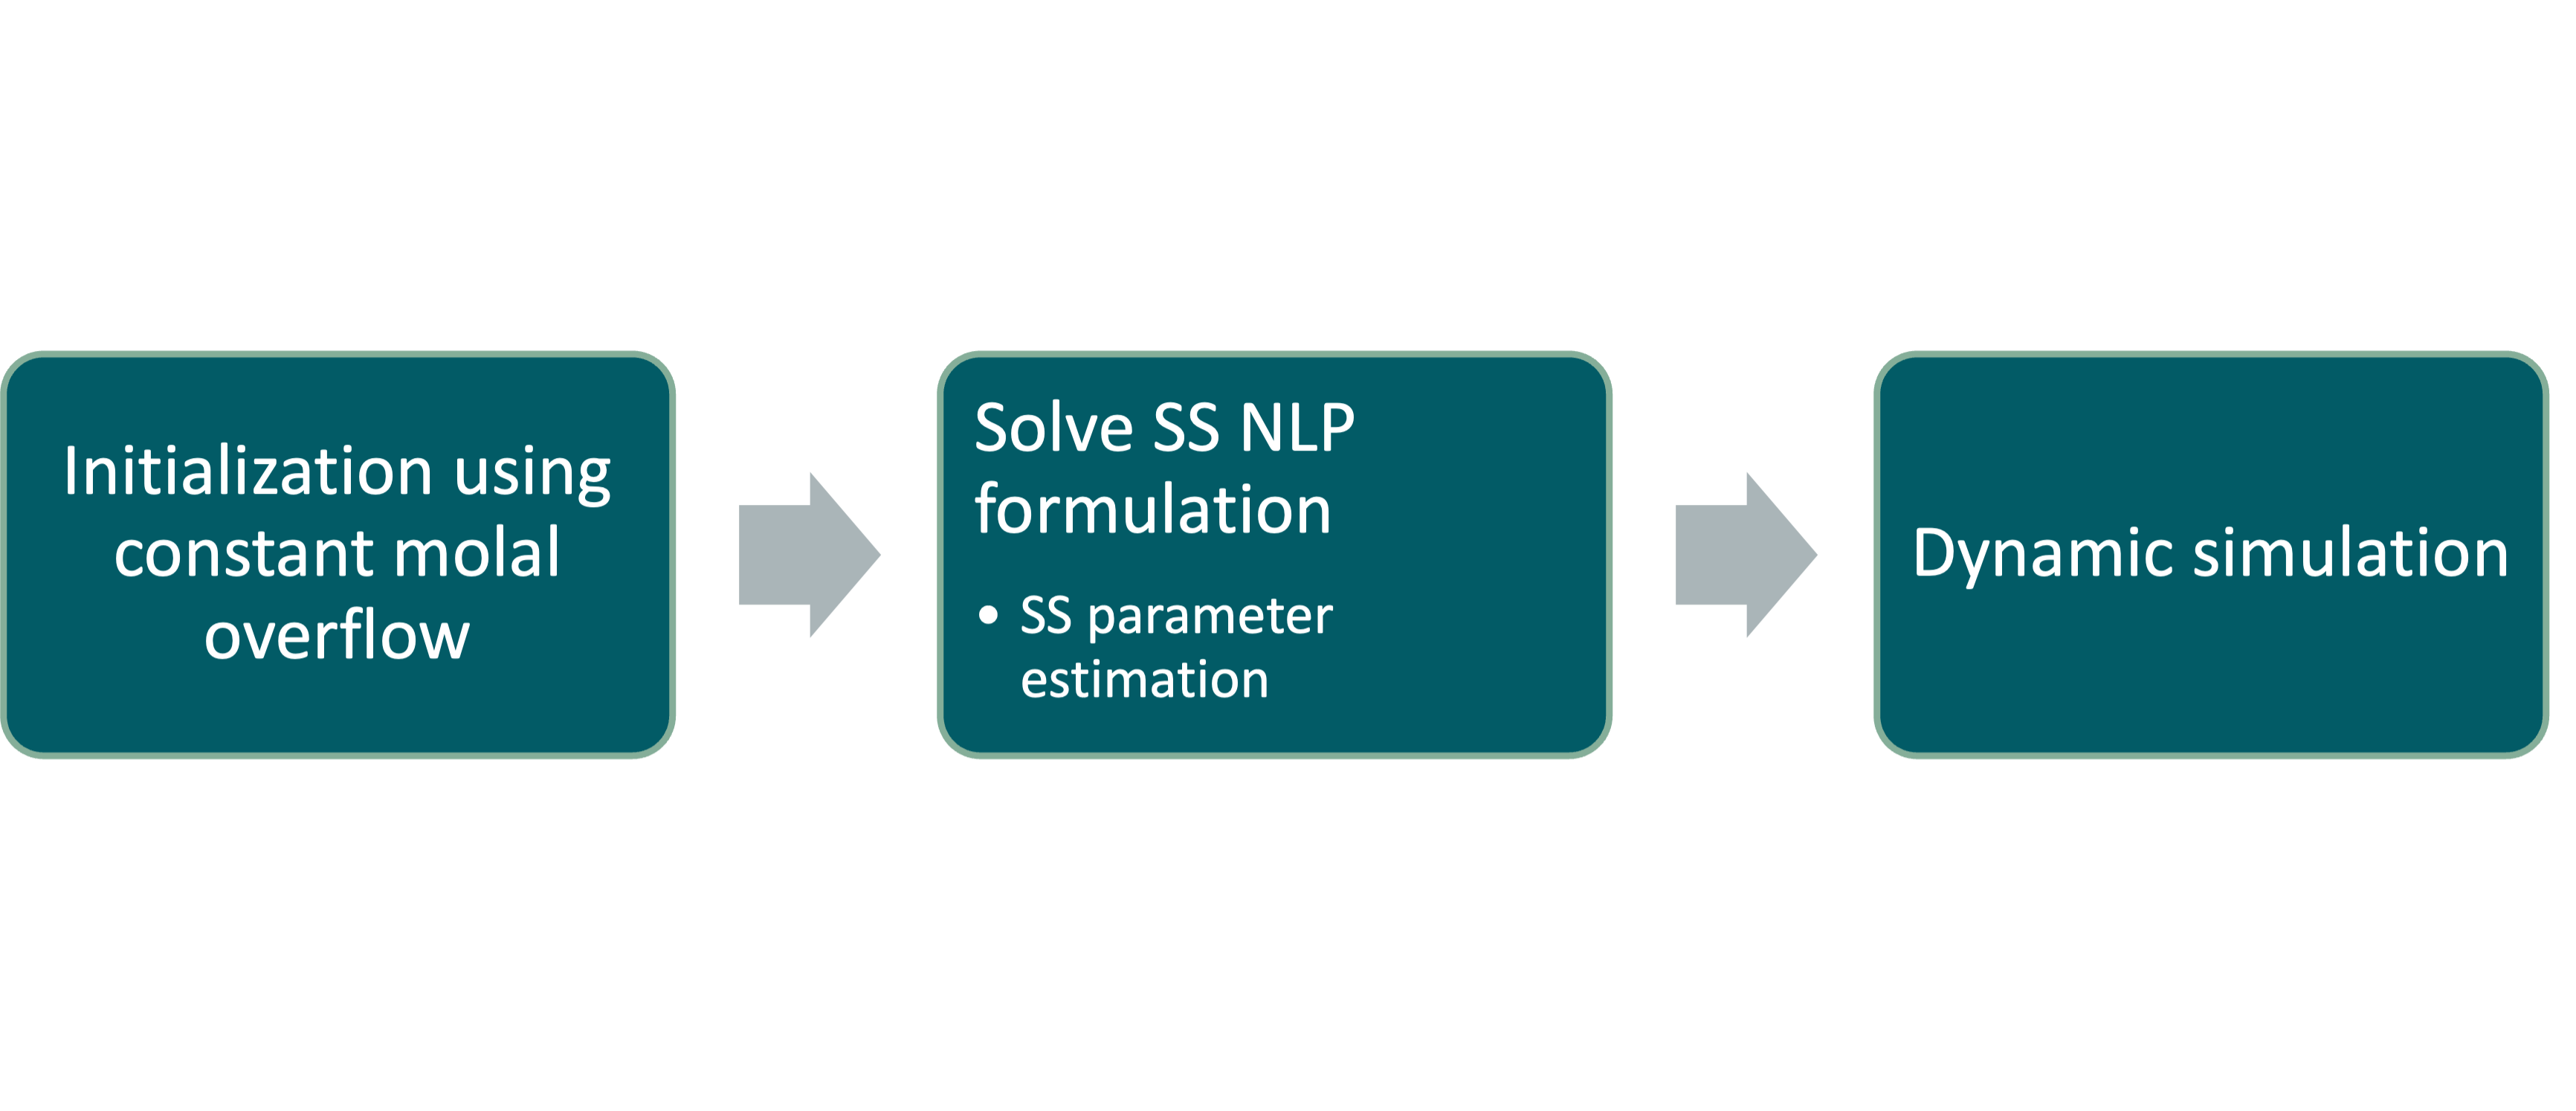
\includegraphics[width=\textwidth]{gfx/Chapter06/simulation_workflow.png}
    \caption{Schematic of the workflow for aligning the distillation simulation to experiments.}
    \label{fig:simulation_workflow}
\end{figure}

To initialize  the simulation, only the component material balances and pressure balances were solved. The constant molal overflow assumption was used, which states that there is constant liquid flow in the stripping and rectifying section respectively as well as constant vapor flow. 

Given the initialization, the full steady state simulation was then solved and used to generate the nominal values for steady state parameter estimation to the experimental data. The full list of estimated parameters can be found in Table \ref{tab:param_estimation}. Note that, while the condenser duty during dynamic simulation was fixed at the value from steady state parameter estimation, the reboiler duty was a manipulated variable; therefore, the steady-state estimated value of the reboiler duty served as an initial condition. The objective of the parameter estimation was to minimize the $L_1$ error between the simulation and experimental temperatures on stages 10, 22 and 35, as these stages were shown to be sensitive to changes in the parameters. Therefore, the parameter estimation problem was formulated as:
%  The $l_1$ norm was chosen due to its improved  handling of outliers \cite{Safdarnejad2016}.
\begin{subequations}
    \begin{align}
        \min_{\boldsymbol \theta_{est}} \sum_{i \in \Gamma} \lVert T_i-T_i^{exp}\rVert_2 + w_p \lVert \Delta P^{exp} - \Delta P \rVert_2 \\
        s.t. \;\; 0 = \mathbf g(\mathbf X, \boldsymbol \theta)
    \end{align}
\end{subequations}
where $\mathbf X$ are the state variables in Table X  and $\boldsymbol \theta = \{\boldsymbol \theta_{est}, \boldsymbol \theta_{const} \}$.  $\boldsymbol \theta_{est}$ are the parameters to be estimated in Table \ref{tab:param_estimation} and $\boldsymbol \theta_{const}$. $\Delta P$ is the column pressure drop, and $w_p$ is a weighting for pressure drop objective, set nominally to 100.  $\mathbf f$ is the system of equations represented by equations in section \ref{sec:distillation_model} with all derviatives set equal to zero. 
% \{\mathbf x, \mathbf y, \mathbf T, \mathbf L, \mathbf n\}$ 
\begin{sidewaystable}[]
    \centering
    \caption{Parameters of the distillation column model estimated using experimental data. Estimates of the reboiler and condenser duties were made using the nominal values from the steady-state simulation.}
    \begin{tabular}{cccc}
        \textbf{Parameter} & \textbf{Description} & \textbf{Initial Guess} & \textbf{Estimated Value}  \\
        \hline
         $\alpha_{strip}$ & Murphree efficiency in stripping section &  0.5 & 0.48 \\ 
         $\alpha_{rect}$ & Murphree efficiency in rectifying section & 0.5 & 0.1 \\
         $\Delta P_{rect}$ & Pressure drop in rectifying section &  $\Delta P_{tot}/N$ & 0.96 mbar \\ 
         $\Delta P_{strip}$ & Pressure drop in stripping section &  $\Delta P_{tot}/N$ & 0.96 mbar \\ 
         $ Q_{reb}$ & Reboiler duty at steady state &  0.25 kW  & 0.267 kW  \\
         $ T_{cond}$ & Condenser temperature at steady state &  333 K  & 333 K\\
         $ Q_{subcool}$ & Subcooling heat exchanger duty & -0.25  kW & -0.41 kW \\
         \hline
    \end{tabular}
    \label{tab:param_estimation}
\end{sidewaystable}

I used the steady state simulation as the initialization for dynamic simulation. The simulation was stepped forward in thirty second intervals using a sequential approach. 

% In Figure \ref{fig:validation}a, we show that using the estimated parameters with settings from a different day of experiments gives good alignment between simulation and experiment.  An example closed-loop dynamic simulation is shown in Figure Xb, which demonstrates that the dynamic simulation aligns closely to the experimental dynamics. 

% \begin{figure}
%     \subfloat[]{
%         \centering
%         \includegraphics[clip,width=\textwidth]{gfx/Chapter06/2021_11_18_steady_state_temperature.png}
%     }

%     \subfloat[]{
%         \centering
%         \includegraphics[clip,width=\textwidth]{gfx/Chapter06/2021_11_18_steady_state_temperature.png}
%         \subcaption{}
%     }
%     \caption{Caption}
%     \label{fig:validation}
% \end{figure}

\section{Results}

\subsection{Distillation simulation correlates with experiments}

In order to build a simulation that could be used for examining the effectiveness of multifidelity BO for controller tuning, I aligned the simulation to experimental data collected at BASF. The resulting steady-state simulation after parameter estimation is shown in Figure \ref{fig:estimated}, which aligns well to the experimental temperature profile. I used an average of the experimental stage temperatures over nine hours of steady state experimental data for parameter estimation. 

The simulated steady state temperature profile aligns well with the experimentally measured temperatures. In particular, the simulation is able to capture the rapid change in temperature between stage 10 and 20. However, the temperature of the middle section of the column is significantly lower than the experimentally measured values. This discrepancy could be due to a number of missing phenomena in the simulation including the heaters in the real column used to prevent heat loss from the column. These heaters could potentially increase the temperature of the internals of the column in a nonlinear fashion throughout the column. 

% Figure 3: Steady state simulation
\begin{figure}
    \centering
    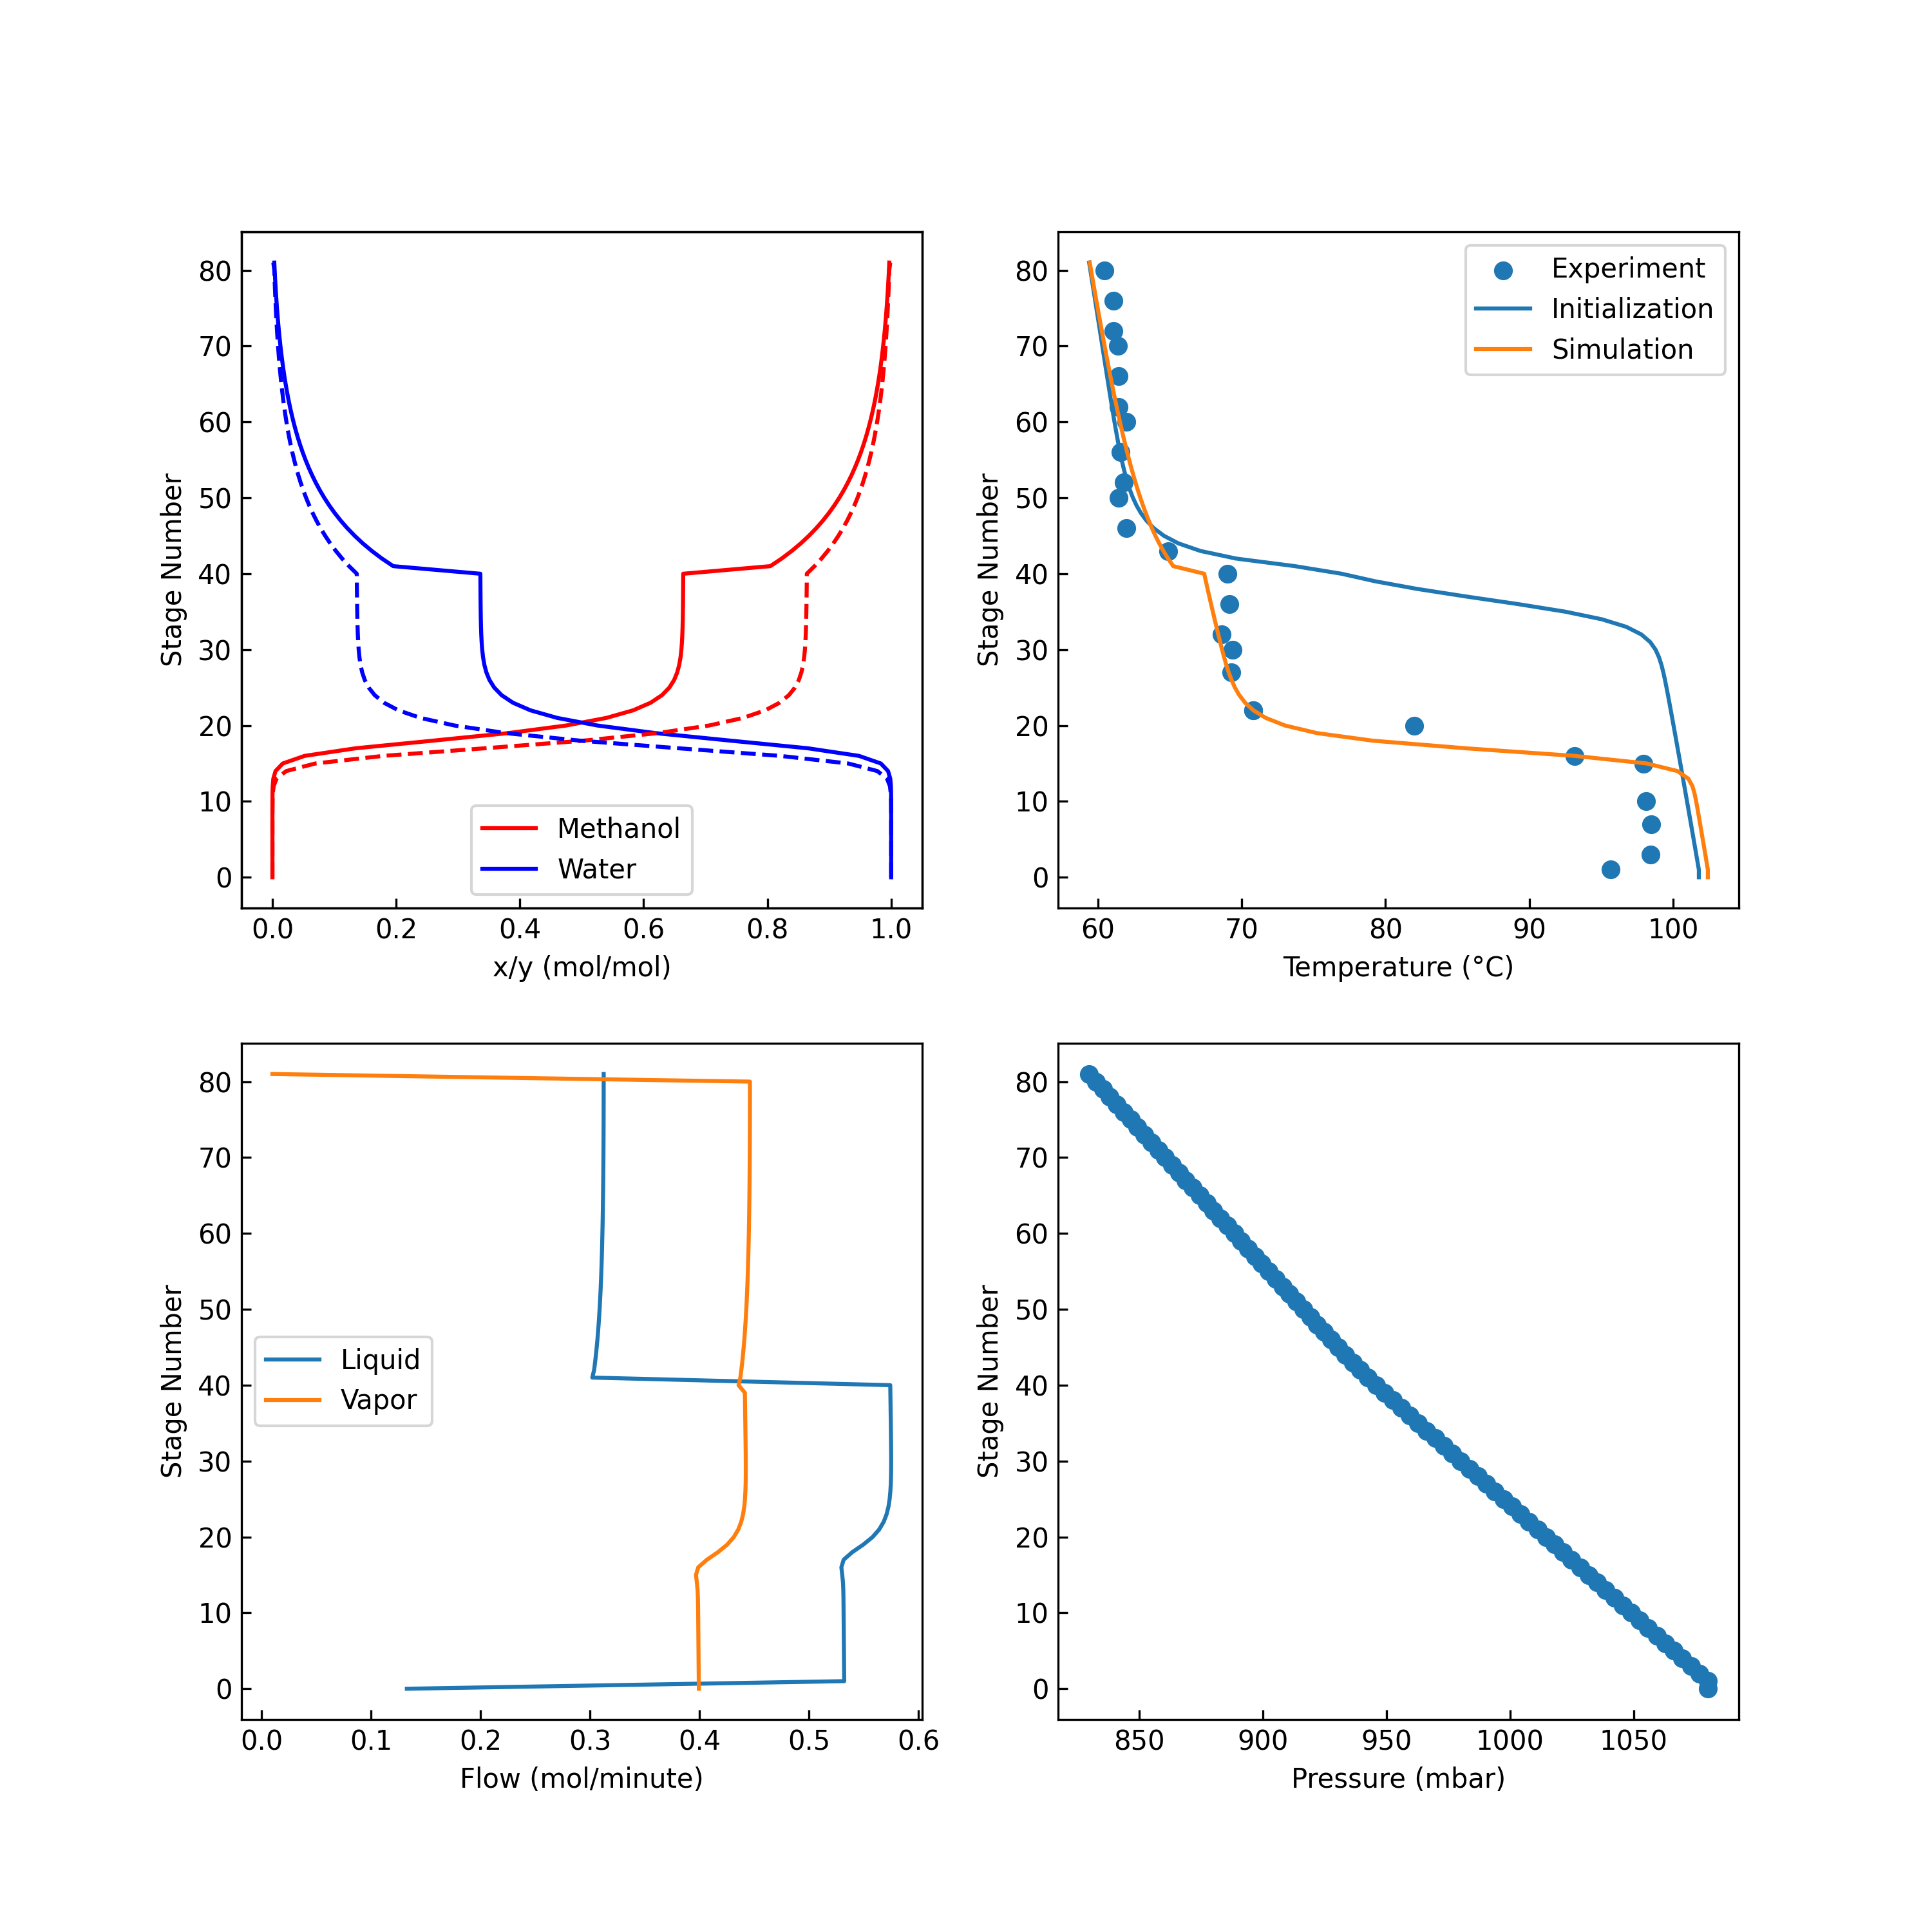
\includegraphics[width=\textwidth]{gfx/Chapter06/2021_11_17_steady_state_estimated.png}
    \caption{Steady state simulation after parameter estimation of a separation of 50/50 methanol-water separation in a distillation column with 80 bubble cap trays. \textbf{Top left}: Composition profile of the column with liquid composition in solid lines and vapor composition in dotted lines. \textbf{Top right}: Temperature profile of the simulation and experiments. \textbf{Bottom left}: Flow profile in column. \textbf{Bottom right}: Pressure profile in column.}
    \label{fig:estimated}
\end{figure}

While, the steady state simulation, we found that the dynamic simulation did not fully capture all aspects of the experiments. In particular, the frequency response of the simulation upon a step in reflux rate did not reflect the oscillations seen in the actual experiments. Achieving a perfect match between the experimentally measured values and simulation is difficult, especially when the experiments are measured in closed-loop. However, I proceeded forward with Bayesian optimization given that the simulations captured some aspects of the steady-state and dynamic behavior of the distillation column.
 
% Figure 4: Dynamic simulation
\begin{figure}
    \centering
    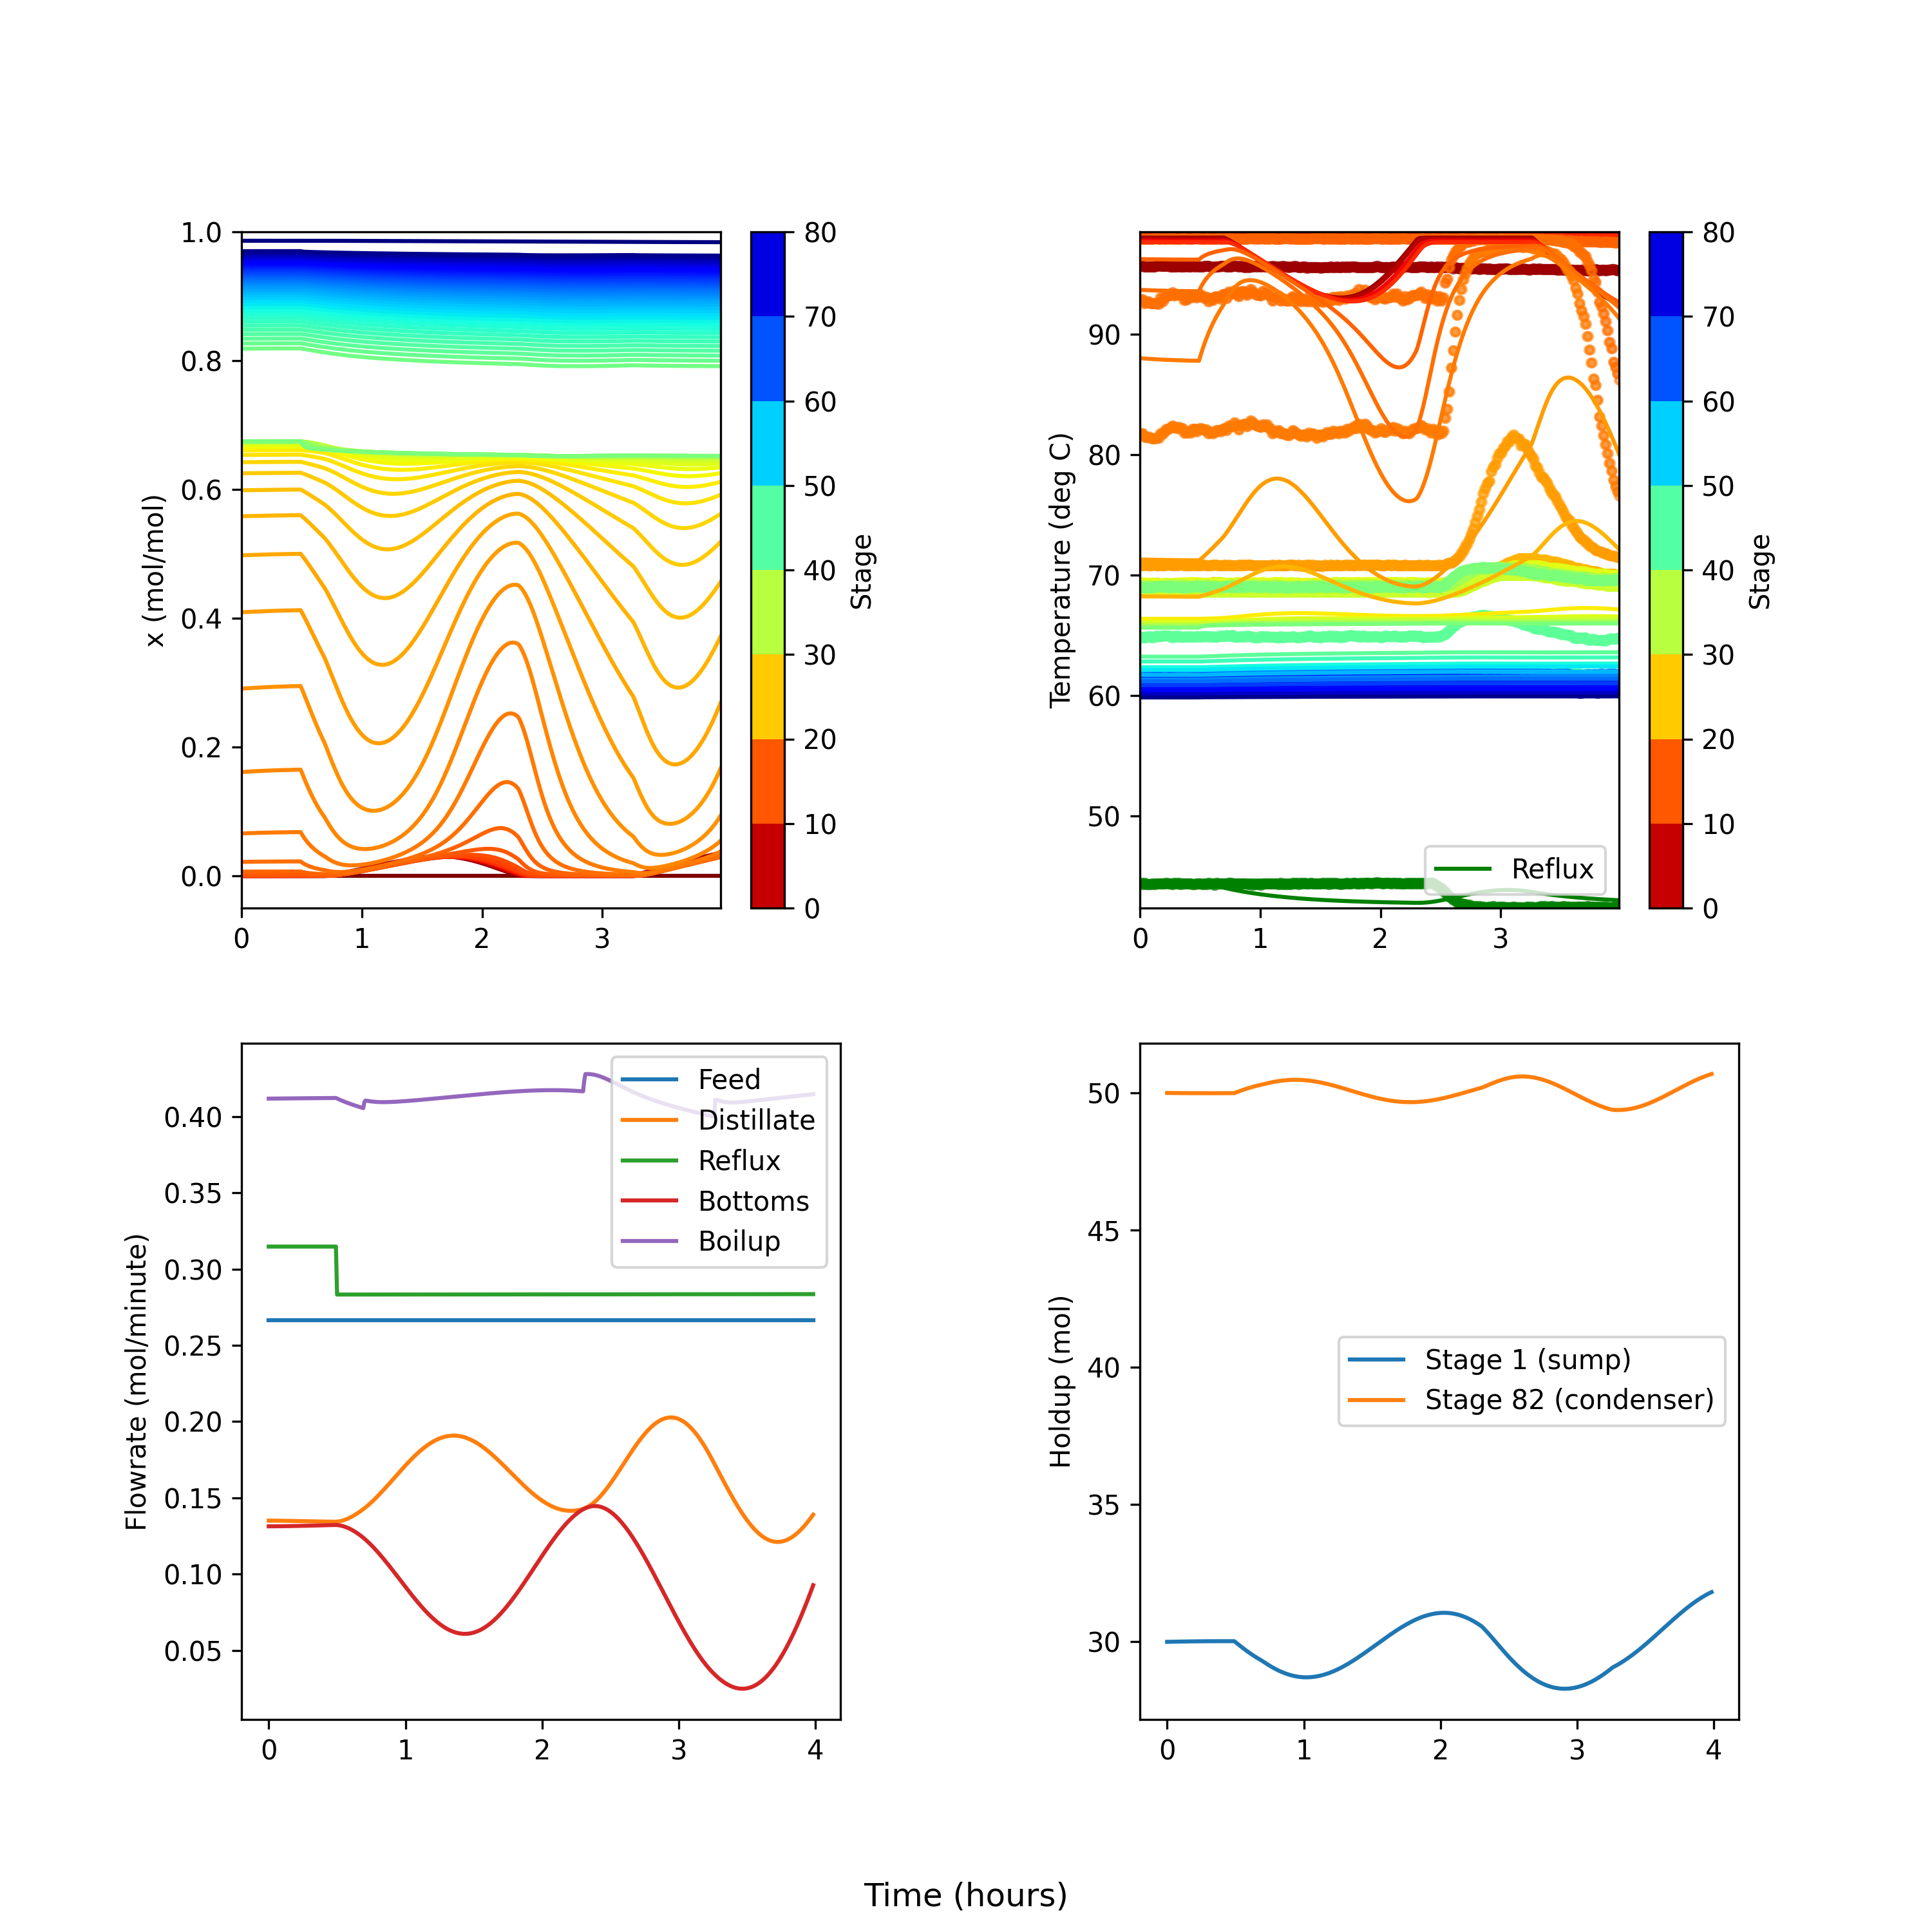
\includegraphics[width=\textwidth]{gfx/Chapter06/2021_11_17_closed_loop_dynamic.png}
    \caption{Dynamic simulation after parameter estimation of a separation of 50/50 methanol-water separation in a distillation column with 80 bubble cap trays. \textbf{Top left}: Liquid composition over time. \textbf{Top right}: Temperature over time. \textbf{Bottom left}: Flow over time \textbf{Bottom right}: Holdups in condenser and reobiler.}
    \label{fig:dynamic_nominal}
\end{figure}


\subsection{Optimization of controller parameters}

To analyze the performance of ControlBO, I analyzed the performance of ControlBO wih and without a multifidelity model. Additionally, I observed that some simulations fail, so I evaluatd it was optimal to use all data by setting large objective values for failed simulations ("All Data" or simply ignore these simulations ("Success only").  Figure \ref{fig:hypervolume_comparison} shows the hypervolume with respect to a fixed reference point during the tuning experiments. As noted in Chapter \ref{ch:summit}, hypervolume is a measure of the volume dominated by the Pareto front; larger hypervolumes correspond with more optimal solutions discovered (i.e., minimal IAE and CM). Note that the disturbance variables were the feed rate and reflux rate, which were stepped randomly during each tuning experiment. This reflects the actual use case where operators might perform steps on various streams and the tuning system needs to be able to accommodate these external changes. 

All ControlBO were able to find better controller parameters over the course of 20 tuning experiments, improving its approximation of the Pareto front. Furthermore, using the auxiliary data from simulations resulted in faster optimization with optimal tuning parameters being found within 2-3 tuning experiments compared 5-10 for single fidelity. Furthermore, using data from only successfull simulations improved both the single-fidelity and multifidelity strategies. This indicates that methods that can automatically classifiy success of simulations could improve the performance of ControlBO in the future.

% Figure 5: Hypervolume vs iterations
\begin{figure}
    \centering
    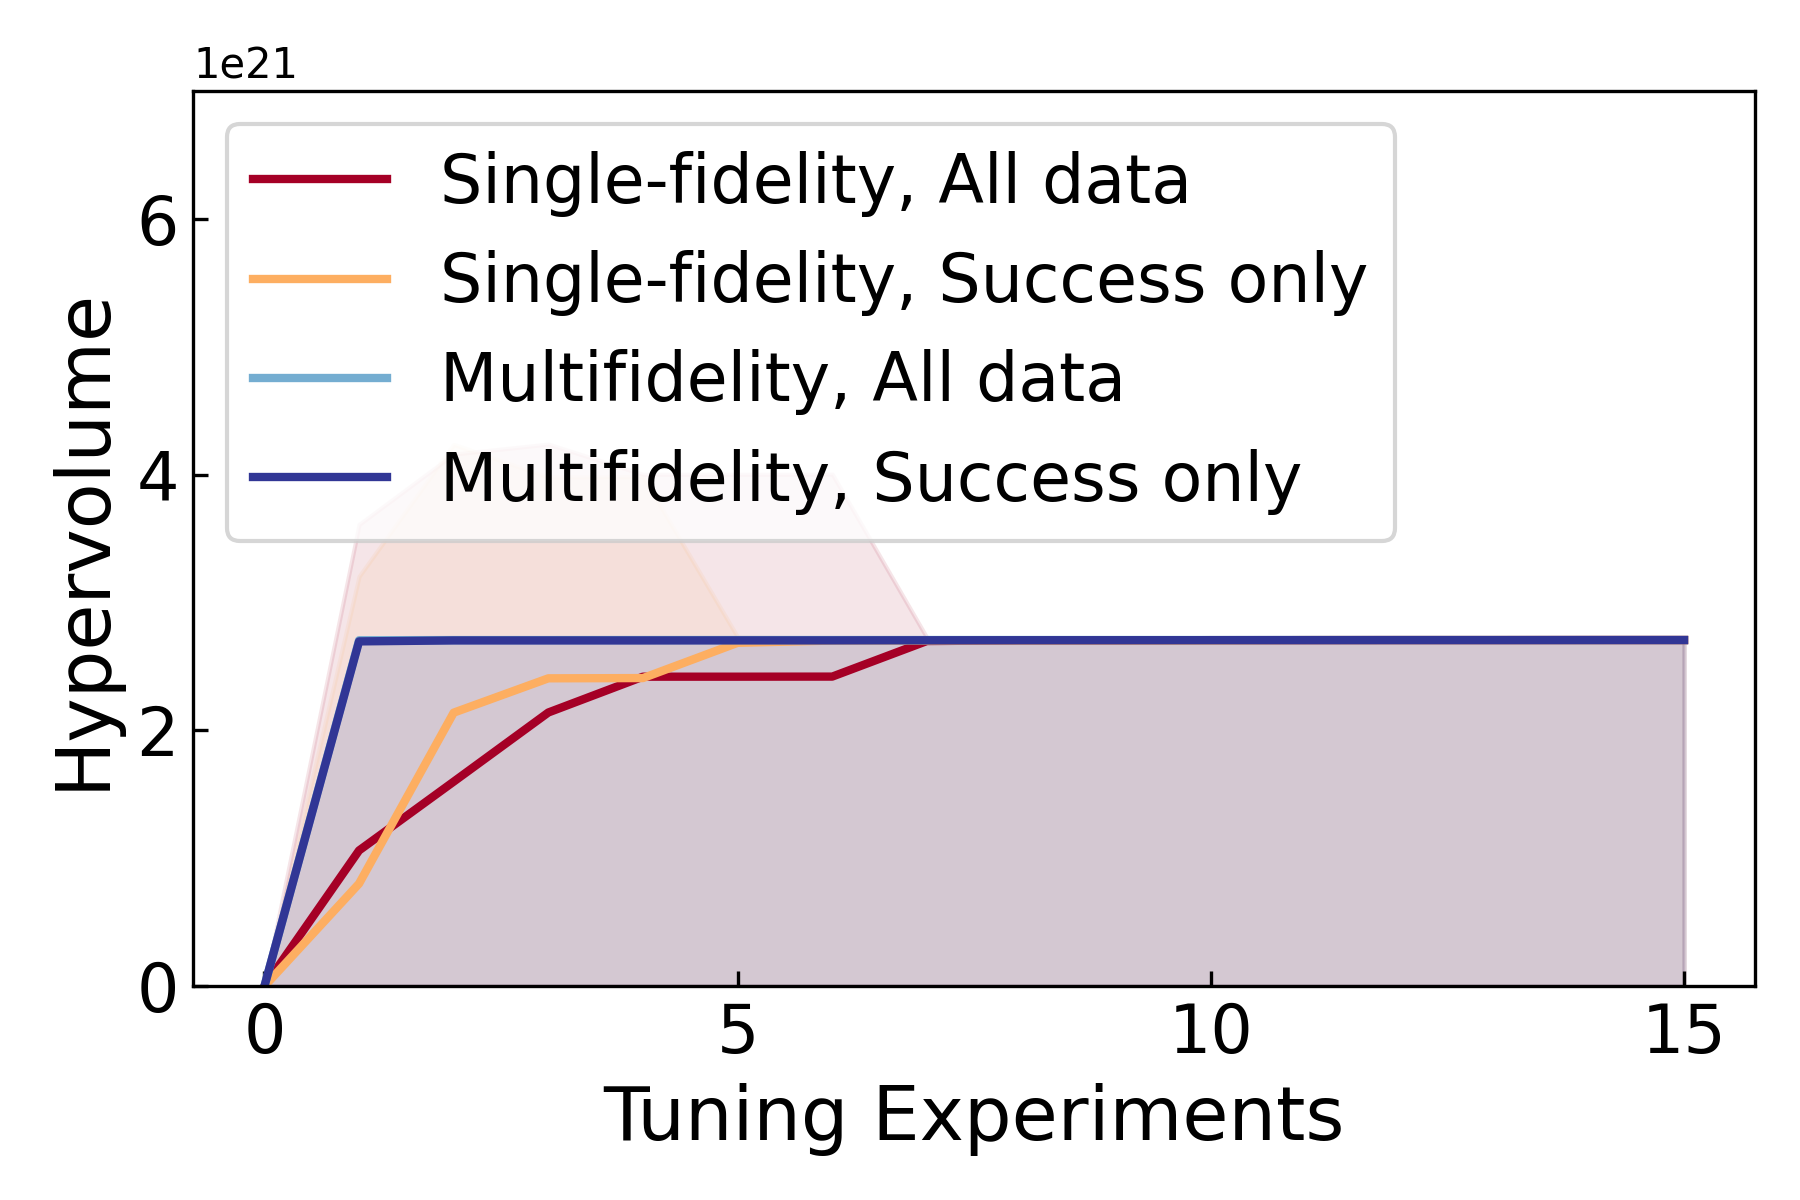
\includegraphics[width=\textwidth]{gfx/Chapter06/hypervolume_comparison.png}
    \caption{Hypervolume trajectory of a single optimization run. Hypervolume is a measure of the volume dominated by the Pareto front; larger hypervolumes correspond with more optimal solutions discovered.}
    \label{fig:hypervolume_comparison}
\end{figure}

In Figure \ref{fig:comparison_controlbo}, I create a performance metric to compare the final tuning of each optimization strategy. The metric is as follows:  

\begin{equation}
\begin{split}
    Objective = w_1 IAE_{sump} + w_2 IAE_{condenser} +  & \\ w_3 IAE_{composition} +  w_4 CM_{sump} + & \\  w_5 CM_{condenser} + w_6 CM_{composition}
\end{split}
\end{equation}

where $w_i$ is a weighting which is the inverse of the maximum value of each objective. The single-fidelity strategy obtains the best overall tuning despite requiring more tuning experiments to achieve this performance. 

\begin{figure}
    \centering
    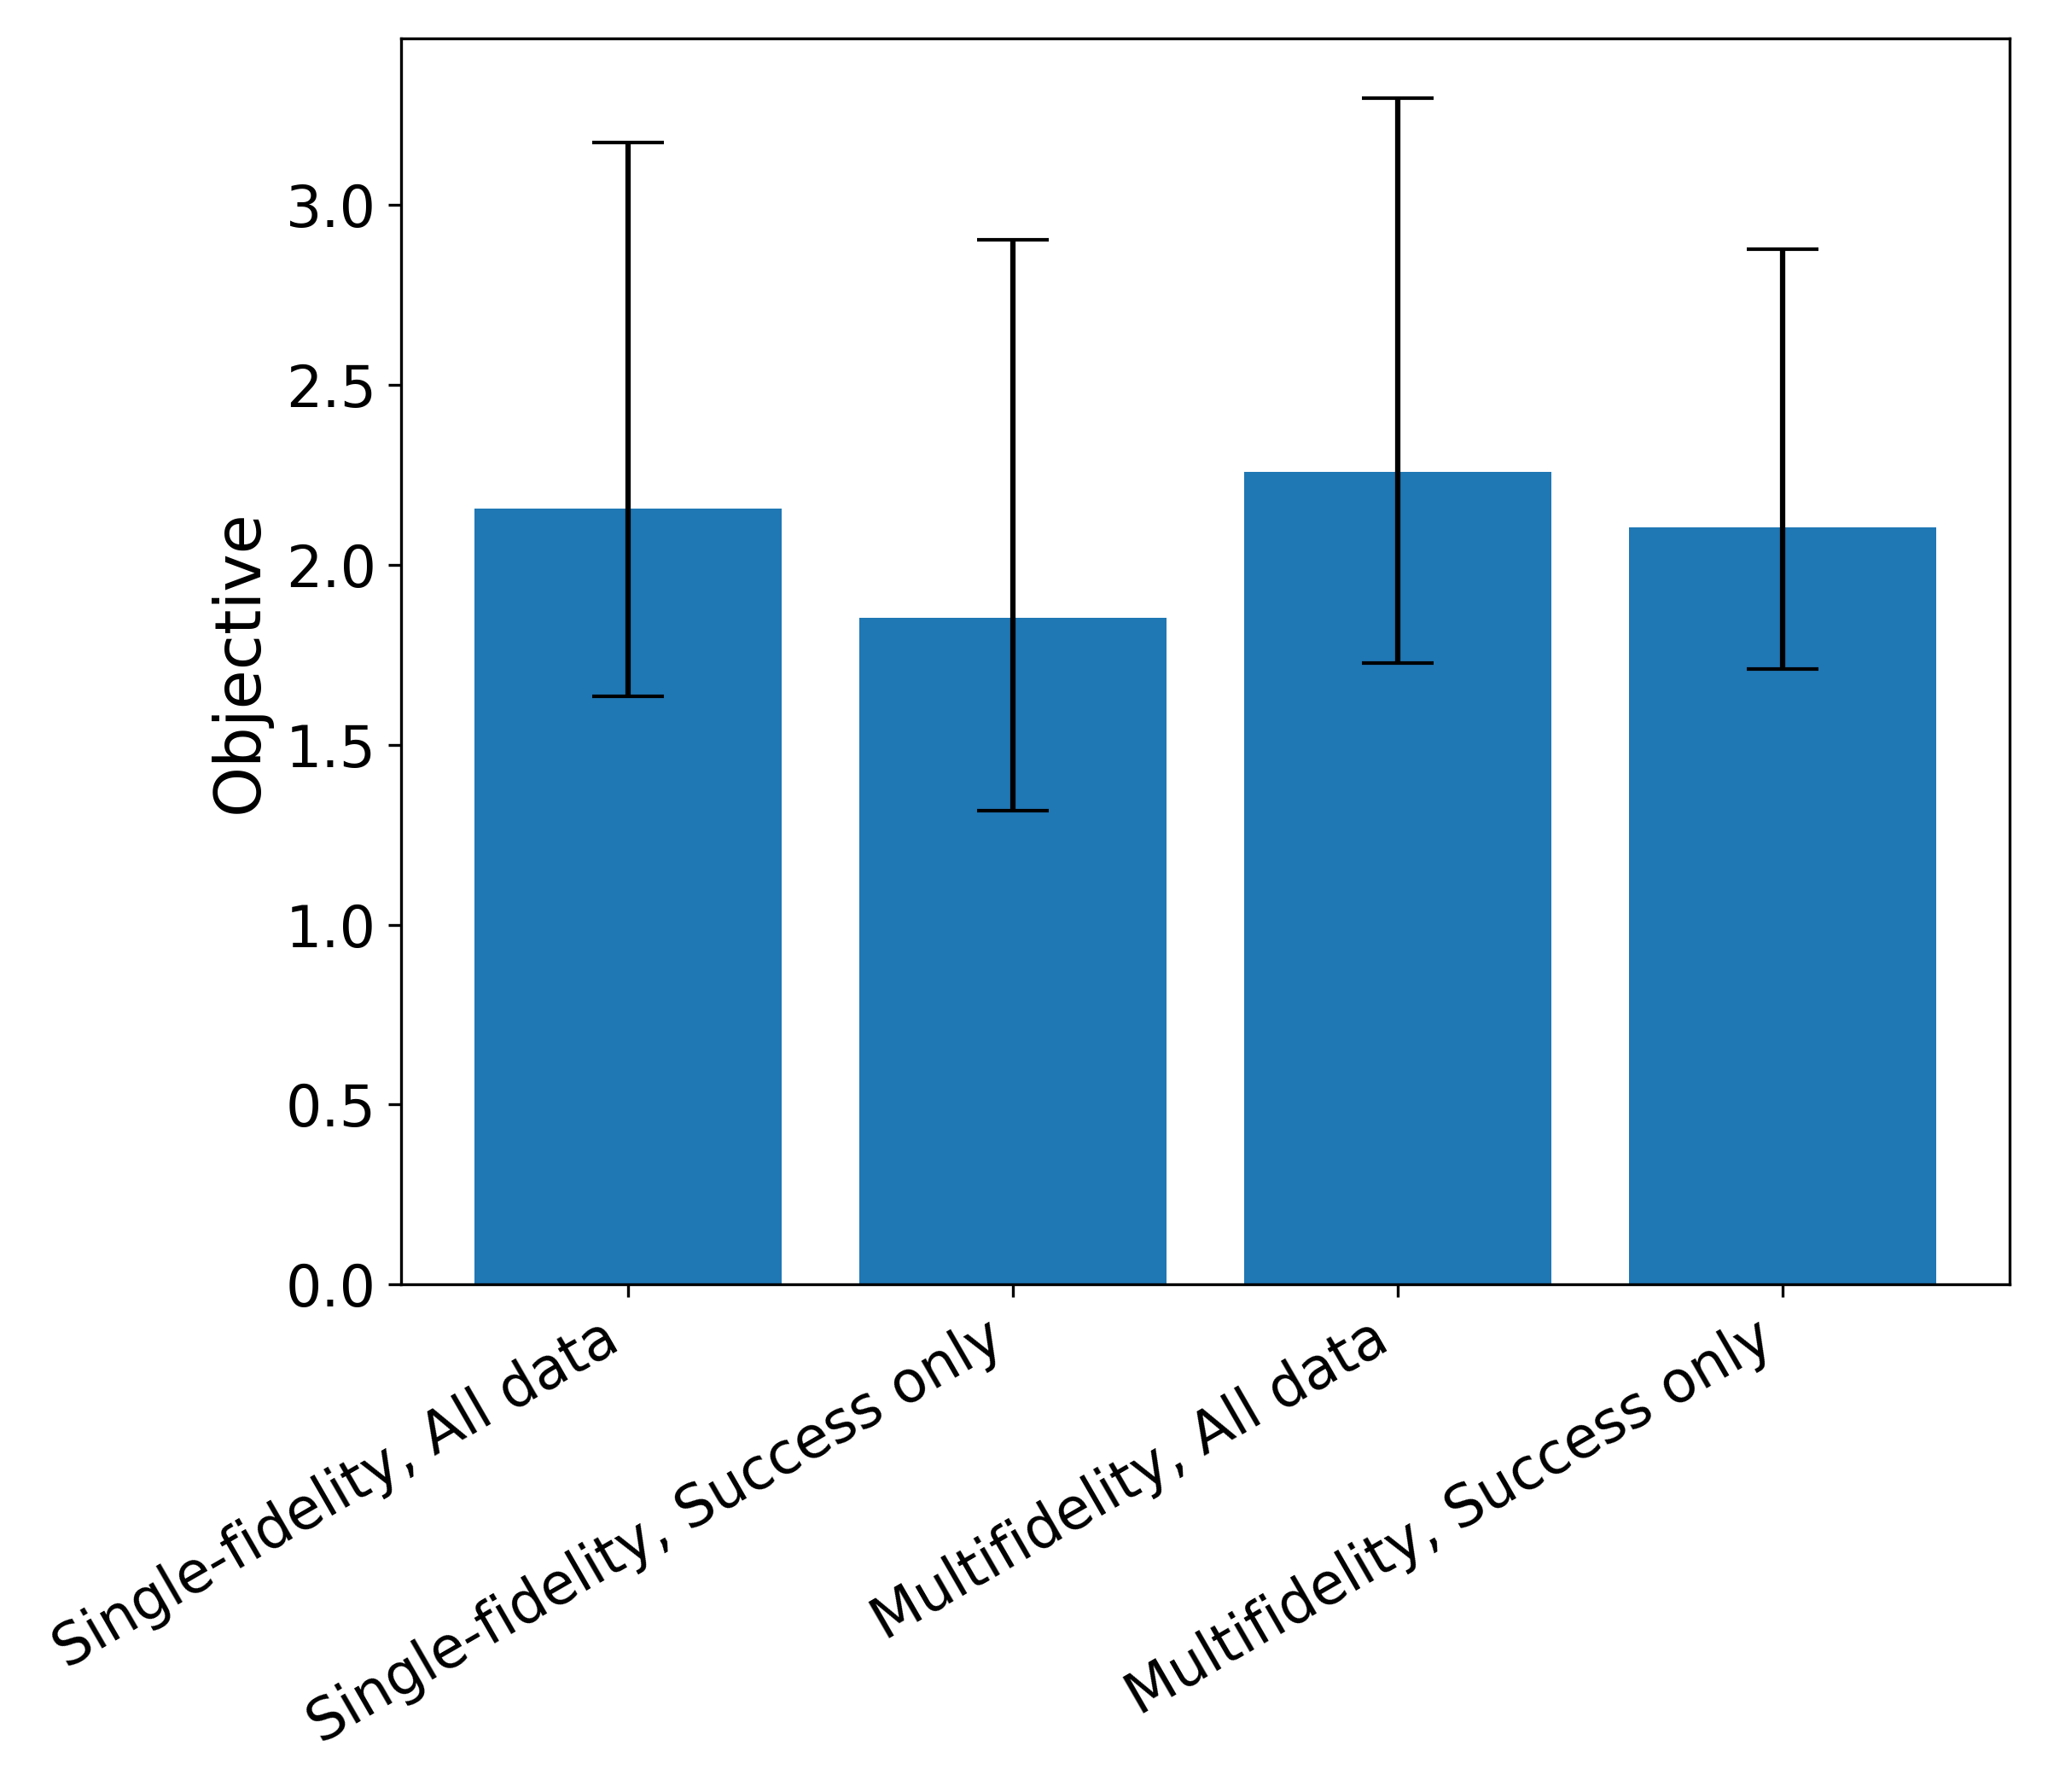
\includegraphics[width=\textwidth]{gfx/Chapter06/comparison.png}
    \caption{Comparison of ControlBO with/without multitask model and with/without using all data.}
    \label{fig:comparison_controlbo}
\end{figure}

% Subsequently, I tested whether a multitask model trained on 100 tuning experiments from an auxiliary simulation could improve the speed at which tuning occcurs. The multitask model should have better correlation but it doesn't. The success classifier doesn't help at all. This is likely due to the fact that the model is able to optimize the controller parameters without many changes and can find the best attainable parameters in  a few iterations. In other words, the problem is made easier by the poor quality of the distillation model.


\section{Conclusion}

Here, I compared several appraoches to optimizing control systems distillation columns using Bayesian optimization. I developed a simulation of a distillation column, which I aligned to experiments conducted by BASF. Subsequently, I used this simulation to explore the use of ControlBO, a multifidelity, multiobjecitve Bayesian optimization strategy designed for controller tuning. I found that ControlBO could find optimal tuning parameters within twenty experiments. Using ControlBO in multifidelity mode (i.e., with a multitask model) improved the speed of optimization but did not result in better final tuning. Additionally, using only data from successful simulations improved tuning performance.

This work is a first step in the direction of leveraging a combination of simulation and machine learning to accelerate controller tuning. However, There are significant challenges both in developing a robust dynamic simulation of a distillation column and applying Bayesian optimization to controller tuning. My distillation simulation does not take into account dynamic pressure changes, which do occur in actual laboratory distillation columns. While our experimental data suggest that pressure drop changes are small in the specific case study due to the use of a vacuum pump for control, more general application of this approach would require taking into account these pressure dynamics to accurately represent dynamic behavior. Similarly, our Bayesian optimization strategy only uses simple time-domain controller performance metrics, while frequency domain performance metrics might give more transferable results. Additionally, we test only on simulations here, but deployment on a real distillation column would be key to verifying the viability of our approach.

